\documentclass[border=10pt]{standalone}

\usepackage{tikz}
\usepackage{tikzsymbols}
\usetikzlibrary{calc,patterns,shapes.geometric}

\def\centerarc[#1](#2)(#3:#4:#5){\draw[#1] ($(#2)+({#5*cos(#3)},{#5*sin(#3)})$) arc (#3:#4:#5);}

\begin{document}
	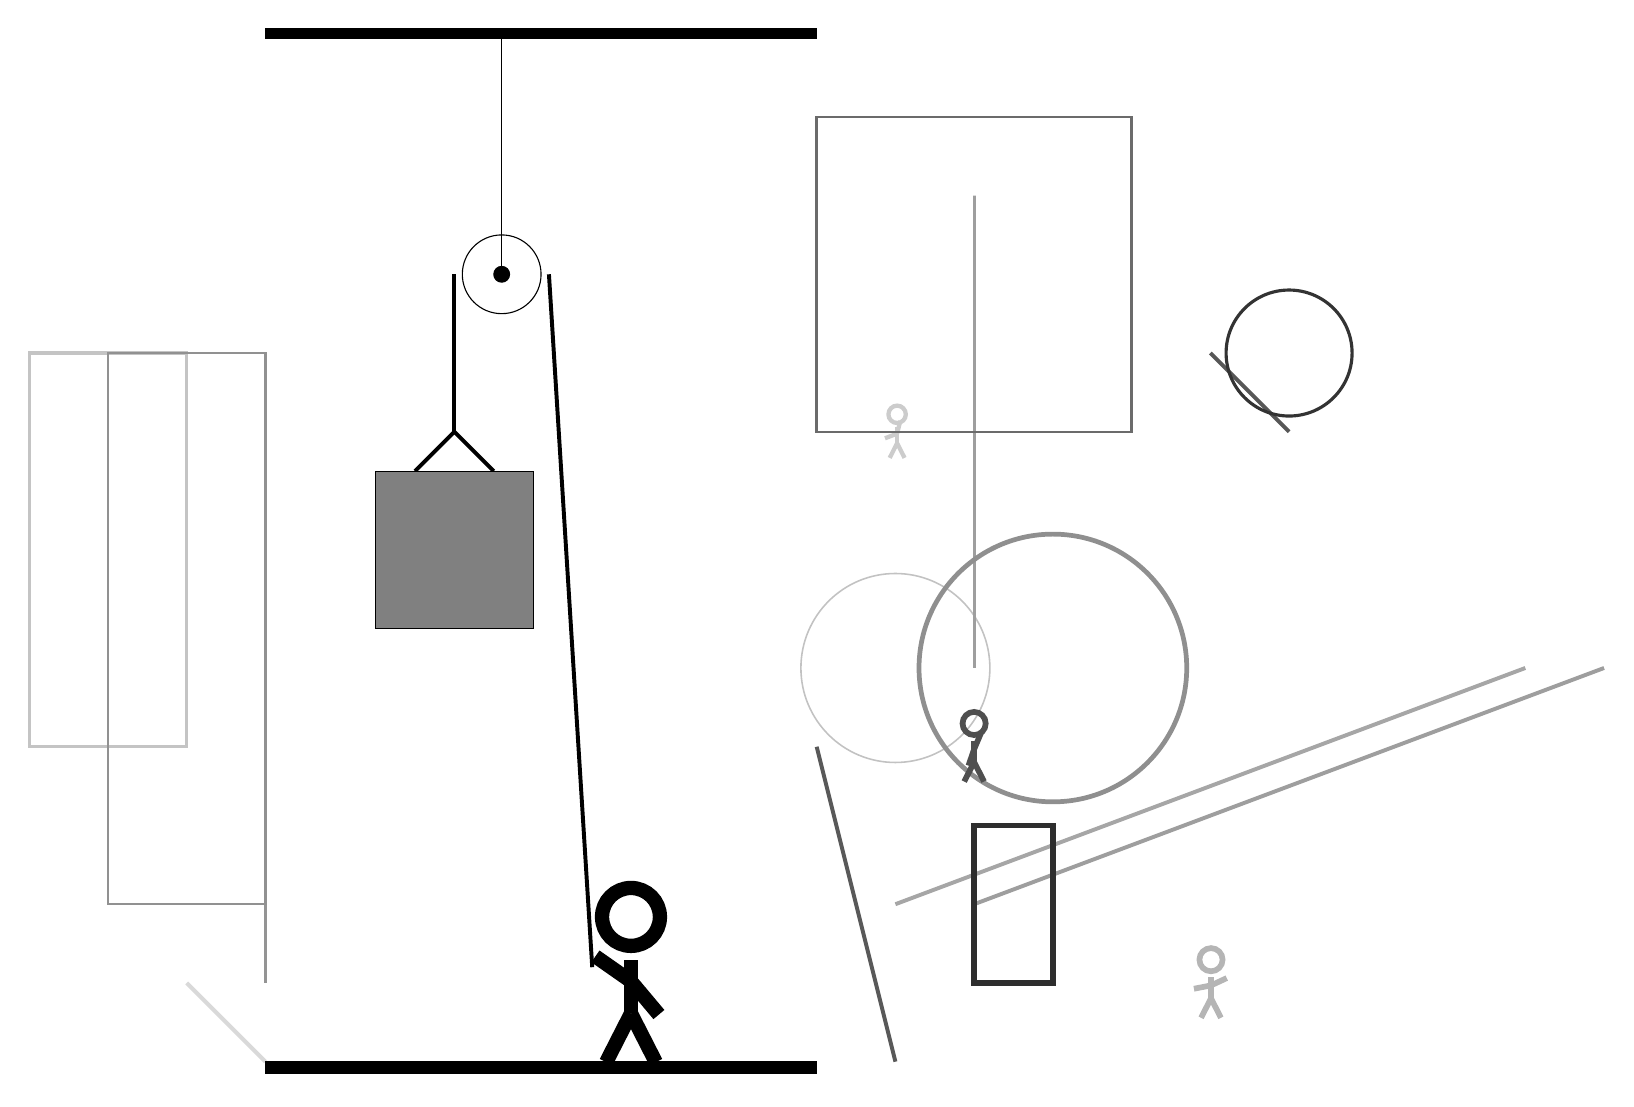
\begin{tikzpicture}
		%%%%% START %%%%%
		
		\draw[fill=black] (-2, 10) rectangle (5, 10.125);
		
		\draw (1, 7) circle (0.5);
		\draw[fill=black] (1, 7) circle (0.1);
		\draw (1, 10) -- (1, 7);
		
		\draw[line width=0.5mm] (-0.1, 4.5) -- (0.4, 5.0) -- (0.9, 4.5);
		\draw[fill=black!50] (-0.6, 4.5) rectangle (1.4, 2.5);
		
		\draw[line width=0.5mm] (0.4, 7) -- (0.4, 5.0);
		\centerarc[line width=0.5mm](1, 7)(0:180:0.6);
		\draw[line width=0.5mm](1.6, 7) -- (2.15, -1.8);
		
		\node at (2.6, -1.9) {\Strichmaxerl[10][-35][-50]};
		
		\draw[line width=0.5mm, color=black!65](5, 1) -- (6, -3);
		
		\draw[line width=0.4mm, color=black!42] (-2, -2) rectangle (-2, 3);
		\draw[line width=0.4mm, color=black!23] (-3, 6) rectangle (-5, 1);
		\draw [line width=0.2mm, color=black!24](6, 2) circle (1.2);
		\node[line width=0.5mm, color=black!29] at (10, -2) {\Strichmaxerl[4][11][25]};
		\node[line width=0.4mm, color=black!20] at (6, 5) {\Strichmaxerl[3][21][76]};
		
		\draw[line width=0.5mm, color=black!66](10, 6) -- (11, 5);
		\draw[line width=0.4mm, color=black!38] (7, 8) rectangle (7, 2);
		\draw[line width=0.3mm, color=black!58] (5, 5) rectangle (9, 9);
		\draw[line width=0.3mm, color=black!43] (-4, -1) rectangle (-2, 6);
		\draw [line width=0.6mm, color=black!44](8, 2) circle (1.7);
		
		\node[line width=0.2mm, color=black!69] at (7, 1) {\Strichmaxerl[4][71][67]};
		\draw [line width=0.4mm, color=black!80](11, 6) circle (0.8);
		
		\draw[line width=0.5mm, color=black!15](-2, -3) -- (-3, -2);
		\draw[line width=0.5mm, color=black!38](7, -1) -- (15, 2);
		\draw[line width=0.5mm, color=black!35](6, -1) -- (14, 2);
		\draw[line width=0.7mm, color=black!82] (7, 0) rectangle (8, -2);
		
		
		\draw[fill=black] (-2, -3) rectangle (5, -3.15);
		
		%%%%% END %%%%%
	\end{tikzpicture}
\end{document}